\subsection{Optimización con y sin gradientes}

La optimización paramétrica sin el uso de gradientes no es escalable para
problemas con un gran número de variables de diseño, como ocurre por ejemplo en
control óptimo, optimización topológica, o aprendizaje automático.

Los algoritmos libres de gradiente avanzan hacia el óptimo poblando el espacio
de diseño y evaluando la función objetivo en estos puntos, para construir una
representación o estadística del entorno que les permita recorrerlo en una
secuencia de pasos. Sin embargo, al introducir más variables de diseño, el
espacio crece exponencialmente, y por tanto el número de puntos a evaluar. Este
fenómeno se conoce como 'la maldición de la dimensionalidad'.

\begin{figure}[h] \centering
	\centering
	\includesvg[width=0.6\textwidth]{./capitulos/metodologia/images/volume_curse_of_dimensionality_print}
	\caption{Crecimiento exponencial del número de puntos a poblar con el número de dimensiones.}
	\label{fig:hypercube}
\end{figure}

Asumiendo que la evaluación de cada punto tiene un coste computacional no
despreciable, el uso de estos algoritmos se vuelve inviable para problemas con
más de unas pocas decenas de variables de diseño. El volumen de un hipercubo
n-dimensional, que podemos pretender representa nuestro espacio de diseño,
se expresa como:

\begin{equation}
	V = l^n
\end{equation}

donde $l$ es la longitud del lado y $n$ es la dimensión.

Por el contrario, los algoritmos basados en gradientes no requieren poblar el
espacio de diseño para encontrar una dirección hacia el óptimo. Emplean los
gradientes de la funcion objetivo respecto de las variables de diseño como
guía, y su obtención es independiente del número de incógnitas, como veremos
con la diferenciación automática y derivadas adjuntas.

Sin importar la técnica escogida para orientarse en el entorno de diseño, la
trayectoria desde el punto inicial al final crece con la dimensión, pero no de
forma tan drástica. La diagonal de un hipercubo n-dimensional viene dada por:

\begin{equation}
	d = l\sqrt{n}
\end{equation}

Nótese que el aumento no es exponencial con el número de dimensiones, ni tan
siquiera lineal.

Si el número de iteraciones realizadas por el algoritmo de optimización es
proporcional a la longitud del camino entre los puntos inicial y final(óptimo),
entonces el coste computacional se incrementa con la raiz del número de
dimensiones, o variables de diseño.

Esta estrategia permite la optimización de problemas con un gran número de
incógnitas. Por ejemplo, el modelo de lenguaje Llama-3.1-405b de Meta utiliza
405 mil millones de variables \cite{dubey2024llama}, o parámetros como se
conocen en el contexto del aprendizaje automático.

\begin{figure}[h]
    \centering
    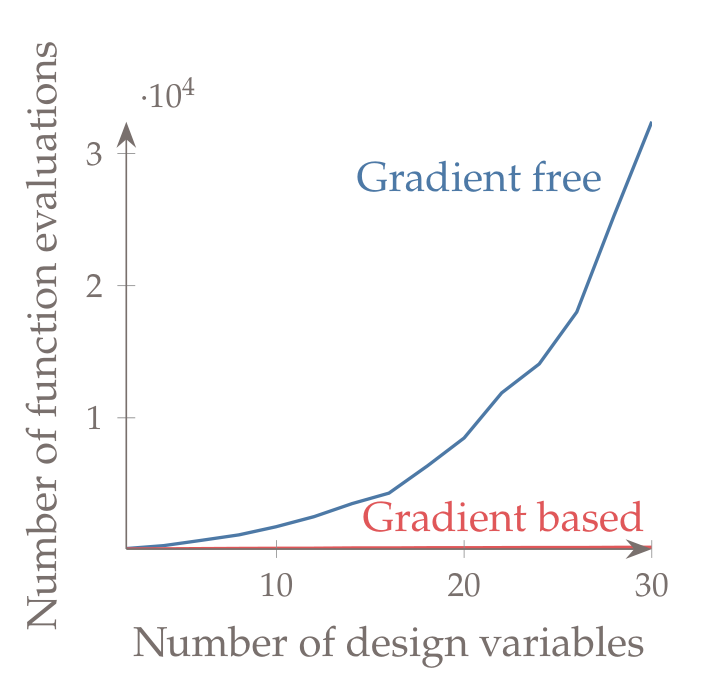
\includegraphics[width=0.4\textwidth]{./capitulos/metodologia/images/gradient_based_vs_gradient_free.png}
    \caption{Los algoritmos de optimización que emplean gradientes escalan mucho mejor con el número de variables de diseño. (Adaptado de Martins y Ning \cite{mdobook}, p. 22)}
    \label{fig:gradient_based_vs_gradient_free}
\end{figure}


\subsection{Restricciones}

La gran mayoría de los problemas en ingeniería requieren el uso de
restricciones en su formulación. Estas restricciones pueden ser de igualdad o
desigualdad y representan limitaciones físicas, económicas o de diseño que
deben satisfacerse durante el proceso de optimización.
